\chapter{MMTSFM: Deep Multimodal Fusion on Frozen Backbones}
\label{cha:method}

This chapter presents the proposed architecture. MMTSFM couples a frozen time-series
foundation model with a frozen video foundation model through two mechanisms that, to the
best of this work's knowledge, have not previously been combined: \emph{selective temporal
interleaving}, which places visual tokens inside the time-series sequence but only within a
short refinement window, and \emph{causal Grassmann mixing}, an $O(L)$ temporal operator
that encodes the transition between hidden states as a subspace on a Grassmann manifold.

The chapter describes the system as built and measured. A subsequent redesign exists on
paper and is discussed as future work in Section~\ref{sec:future}; nothing in this chapter
depends on it.

\section{Overview}
\label{sec:overview}

The model consumes, per entity row, a 672-step normalised power history, fourteen covariate
channels over history and horizon, and eight satellite frames covering a short recent
window. It emits the full six-hour horizon as nine quantiles in a single forward pass.

The data flow is:

\begin{enumerate}
  \item The power history is patch-tokenised by the \emph{pretrained} Chronos-2 patch
    embedding into $T_{\text{ctx}} = \lceil 672/16 \rceil = 42$ context tokens, plus
    $T_{\text{fut}} = \lceil 12/16 \rceil = 1$ future token. Each covariate channel becomes
    its own token row on the batch axis.
  \item The eight frames are encoded as a \emph{clip} by frozen V-JEPA~2.1 into
    $[B, 4, 196, 1024]$ --- four latent time steps, 196 spatial patches --- and compressed
    by a learned latent summariser into $n_{\text{vis}}$ tokens of width 768
    ($n_{\text{vis}}=1$ for \texttt{uk\_pv}, 2 for \texttt{goes\_pvdaq}).
  \item A multimodal embedding layer adds modality, segment, token-type, entity and rotary
    positional information.
  \item The fusion mode determines where visual tokens enter: as additional batch rows
    (late fusion) or woven into the temporal sequence (interleaved).
  \item Twelve Chronos-2 encoder blocks process the result, each applying temporal mixing,
    group self-attention across the batch axis, and a feed-forward layer.
  \item The output head decodes the final future positions into nine quantiles per horizon
    step and inverts the normalisation.
\end{enumerate}

Figure~\ref{fig:architecture} shows the assembled system.

\begin{figure}[p]
\centering
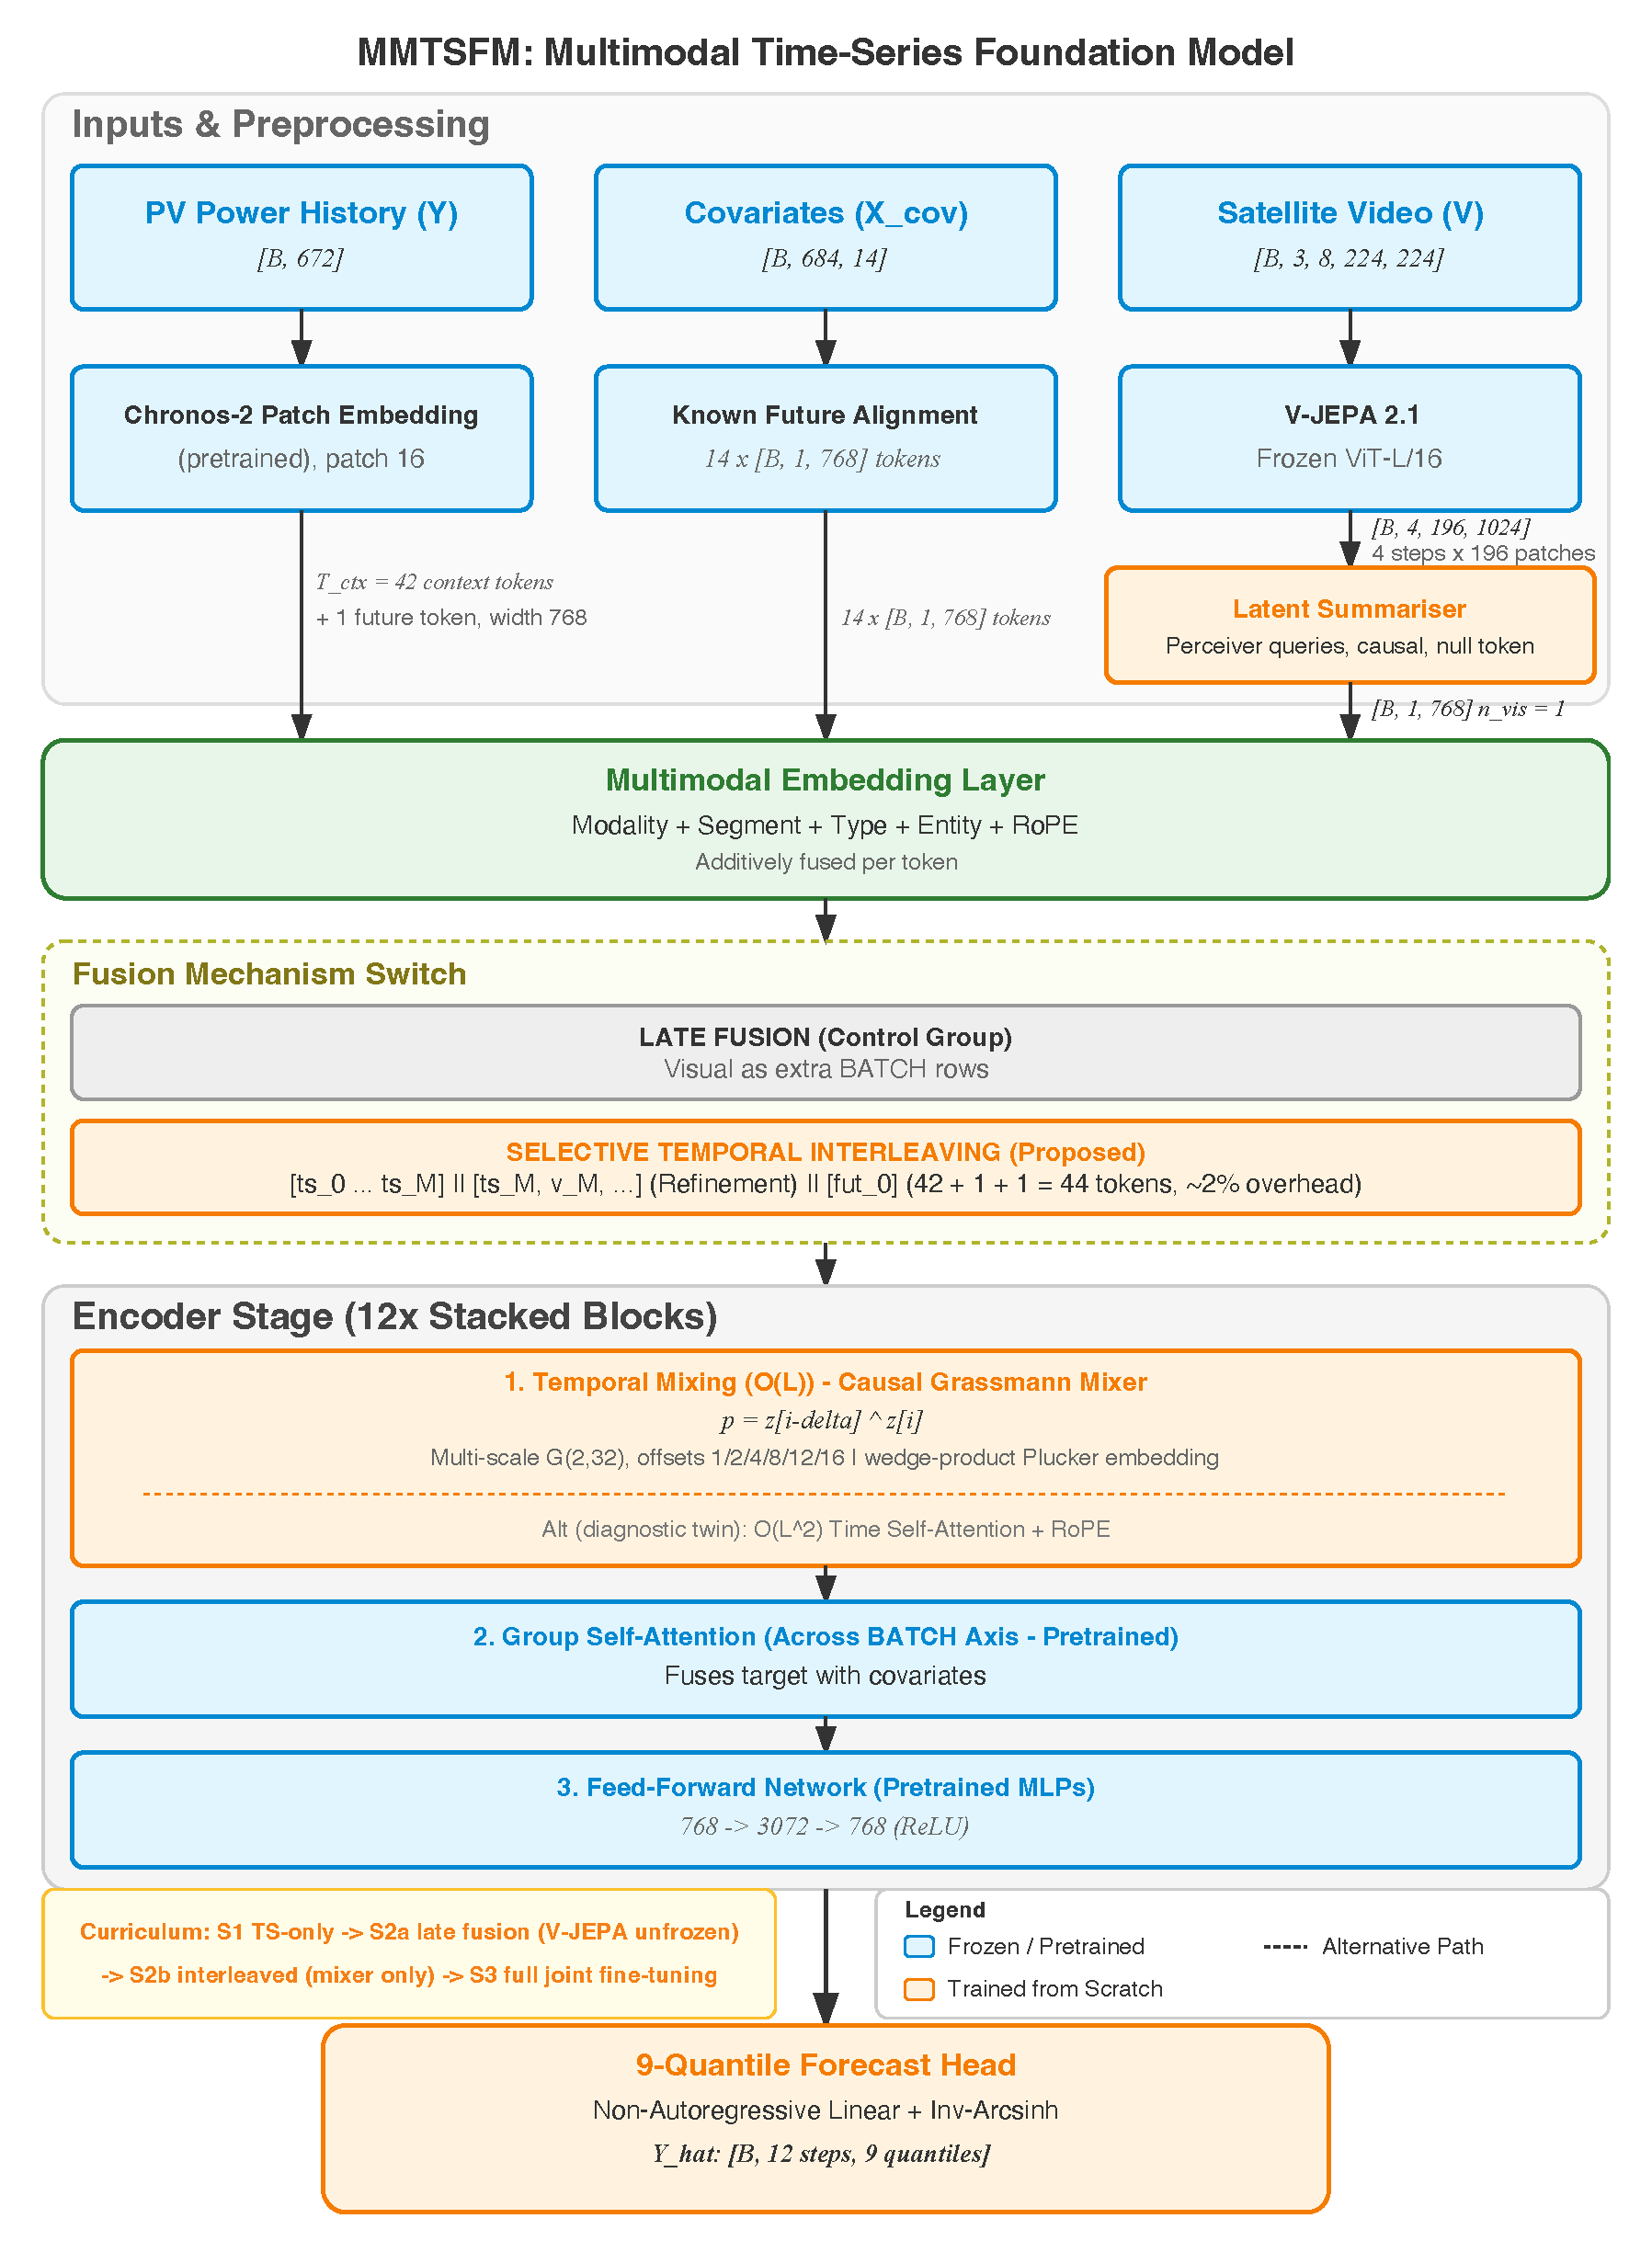
\includegraphics[width=\textwidth]{figures/mmtsfm_architecture.pdf}
\caption{MMTSFM as assembled, for \texttt{uk\_pv}. Cool boxes are pretrained or frozen;
warm boxes are trained from scratch --- the latent summariser, the fusion interface, the
Grassmann mixer and the quantile head are the only newly initialised components. Tensor
shapes are annotated on the edges.}
\label{fig:architecture}
\end{figure}

\subsection{Shapes, worked through}

Table~\ref{tab:shapes} traces one \texttt{uk\_pv} sample from input to output. Tracing shapes
explicitly is worth a page here because two of the design's least obvious properties --- the
aggressive patch compression of the numerical stream, and the extreme compression of the
visual stream --- are invisible in prose and immediate in a shape table.

\begin{table}[h!]
\centering
\small
\begin{tabular}{l l l}
\hline
\textbf{Stage} & \textbf{Shape} & \textbf{Note} \\
\hline
Power history & $[B, 672]$ & 14 days at 30-min cadence \\
After patch embedding & $[B, 42, 768]$ & $\lceil 672/16 \rceil$ tokens; one token
$\approx$ 8 h \\
Future positions & $[B, 1, 768]$ & $\lceil 12/16 \rceil$ \\
Covariates & $[B, 684, 14]$ & history $+$ horizon \\
Covariate token rows & $14 \times [B, 1, 768]$ & one batch row per channel \\
\hline
Frames & $[B, 3, 8, 224, 224]$ & 8 frames over a 6-hour window \\
After V-JEPA & $[B, 4, 196, 1024]$ & tubelet stride 2; 4 latent steps \\
After latent summariser & $[B, 1, 768]$ & $n_{\text{vis}} = 1$ \\
\hline
Interleaved sequence & $[B, 44, 768]$ & $42 + n_{\text{vis}} + T_{\text{fut}}$ \\
After 12 encoder blocks & $[B, 44, 768]$ & shape preserved \\
Output head & $[B, 12, 9]$ & horizon $\times$ quantiles \\
\hline
\end{tabular}
\caption{One \texttt{uk\_pv} sample end to end. Two compressions dominate: 672 timesteps
become 42 tokens, and $4 \times 196 \times 1024$ visual activations become a single
768-dimensional vector.}
\label{tab:shapes}
\end{table}

The second compression is worth dwelling on, because it is a candidate explanation for any
weak visual contribution. The V-JEPA output contains $4 \times 196 = 784$ patch embeddings of
width 1024; the summariser reduces this to one vector of width 768, a reduction of roughly
three orders of magnitude. Whatever spatial structure the cloud field has --- a front
approaching from the west, a break opening to the south --- must survive that bottleneck to
influence the forecast. The visual token budget sweep specified in
Section~\ref{sec:sensitivity} exists precisely to test whether it does.

\section{Design principle: decoupled resolution}
\label{sec:decoupled}

The two modalities are kept at \emph{different temporal resolutions on purpose}. The
numerical stream carries a long macro-context --- two weeks, spanning many diurnal cycles,
enough to expose seasonality and regime structure. The visual stream carries a short
micro-context at high cadence, covering only the last few hours.

Both alternatives are worse. Resampling a fortnight of satellite frames onto the numerical
grid is computationally prohibitive and mostly redundant, since frames more than a few hours
old carry no information about the coming six hours: cloud fields advect out of the crop.
Resampling the numerical series up to the frame cadence discards the macro-context that
makes the foundation-model backbone useful in the first place. Decoupling keeps each modality
at the resolution at which it is informative, and the cost is that fusion must handle
sequences in which the two streams have incommensurable time bases --- which is exactly what
Section~\ref{sec:interleaving} addresses.

\section{Numerical branch}
\label{sec:numeric-branch}

The backbone is Chronos-2~\cite{chronos2} at its native checkpoint size: $d_{\text{model}}$
768, twelve layers, twelve heads with head dimension 64, feed-forward width 3072, input
patch size 16, nine protocol quantiles, and an inverse-hyperbolic-sine normalisation that
makes series of arbitrary magnitude comparable without per-series statistics.

Because the configured input patch size matches the checkpoint, the patch embedding loads
\emph{pretrained} and transfers; only the nine-quantile output head is reinitialised. This is
a deliberate design constraint rather than a happy accident --- a mismatched patch size would
discard the tokeniser and with it most of the value of the pretrained backbone.

\paragraph{A reproducibility trap worth recording.} The configuration files in this project
nominally specify a smaller model ($d_{\text{model}}$ 512, six layers, feed-forward 2048).
These values are \emph{silently ignored}: loading from a pretrained checkpoint preserves the
checkpoint's architecture, and only the Grassmann-specific fields and the tokeniser
configuration propagate. Any report of this system that quotes the configured dimensions
rather than the checkpoint's is wrong. The failure is silent --- no warning, no shape error
--- and it is the kind of discrepancy that survives a long time in a research codebase.

\paragraph{Covariates.} The fourteen covariate channels enter as separate token rows on the
batch axis, sharing a group identifier with the target row, with their masks set so that
values survive to the encoder. That they genuinely reach the model in both fusion modes was
verified by perturbation: changing a covariate changes the forecast. This is worth
stating because a covariate path that is silently masked out is a common and invisible
failure, and because it is what makes the honest-versus-oracle distinction of
Section~\ref{sec:parity} meaningful.

\section{Visual branch}
\label{sec:visual-branch}

The visual encoder is a frozen V-JEPA~2.1 ViT-L/16~\cite{vjepa2}, applied to the entire
eight-frame clip rather than frame by frame. Tubelet embedding with temporal stride two
yields four latent time steps of 196 spatial patches each, at width 1024. Motion is therefore
encoded \emph{inside} the backbone, and the downstream module only has to perform spatial
compression.

That module is a learned \textbf{latent summariser}: a Perceiver-style cross-attention
block~\cite{perceiver} with a small set of learned queries, applied causally across latent
time, and equipped with a \emph{null token} so that the summariser can represent ``no useful
visual evidence'' rather than being forced to emit a confident summary of an uninformative
sky. It maps $[B,4,196,1024]$ to $[B, n_{\text{vis}}, 768]$.

All domain specialisation lives in this summariser. There is no per-sensor input projection:
the data loader delivers uniformly shaped frames for every plant and source, so the queries
--- and only the queries --- learn what to extract from a satellite crop for the purpose of
forecasting power. This mirrors the adapter-recycling strategy used to specialise frozen
vision-language backbones, and it keeps the number of newly initialised parameters small,
which matters for the curriculum of Section~\ref{sec:curriculum}.

\section{Multimodal embedding}
\label{sec:embedding}

Before fusion, every token receives an additive composition of five embeddings: a
\emph{modality} embedding (numeric or visual), a \emph{segment} embedding (context or
future), a \emph{token-type} embedding (target, covariate or visual), an \emph{entity}
embedding, and rotary positional encoding~\cite{rope} over the temporal axis. Additive
composition keeps the embedding table small and lets the encoder disentangle the factors
linearly.

\section{Fusion}
\label{sec:interleaving}

Two fusion modes are implemented, and the difference between them is the architectural
hypothesis under test.

\paragraph{Late fusion.} The visual summary is passed through a cross-modal adapter and
appended as $N_{\text{soft}}=1$ additional \emph{batch rows} sharing the target's group
identifier. The two modalities therefore meet only in the group-attention operator, once per
block, and never interact along the time axis. This is the standard design and serves as the
control.

\paragraph{Selective temporal interleaving.} Let $T_M = T_{\text{ctx}} - n_{\text{vis}}$. The
encoder input sequence is
\[
  \mathbf{S} =
  \underbrace{[\,\mathrm{ts}_0, \ldots, \mathrm{ts}_{T_M-1}\,]}_{\text{macro: pure time series}}
  \;\Vert\;
  \underbrace{[\,\mathrm{ts}_{T_M}, v_{T_M}, \ldots,
               \mathrm{ts}_{T_{\text{ctx}}-1}, v_{T_{\text{ctx}}-1}\,]}_{\text{refinement: interleaved}}
  \;\Vert\;
  \underbrace{[\,\mathrm{fut}_0, \ldots\,]}_{\text{future}} .
\]
Visual tokens are inserted \emph{only} inside the refinement window. The macro region stays
purely numerical, so its temporal geometry --- the structure the pretrained backbone knows
how to exploit --- is left undisturbed; in the refinement region the two modalities alternate,
so that the temporal operator computes genuinely cross-modal pairs.

The causal access pattern follows from the ordering. A time-series token at position
$T_M+2k$ attends to the full macro history and all previous refinement pairs, but not to the
visual token that follows it; the visual token at $T_M+2k+1$ attends to everything above plus
its own time-series partner. Causality is preserved by construction and requires no masking
special case.

\paragraph{Cost.} Total sequence length is $T_{\text{ctx}} + n_{\text{vis}}$: the overhead is
$n_{\text{vis}}/T_{\text{ctx}}$, proportional to the number of visual tokens rather than to
context length. For \texttt{uk\_pv} this is $42+1+1 = 44$ tokens, roughly two percent. Longer
numerical contexts make the ratio smaller, not larger --- which is the opposite of the scaling
behaviour of full cross-attention between two long sequences, and is the practical argument
for the design.

\section{Temporal mixing: causal Grassmann flow}
\label{sec:grassmann}

Each encoder block begins with a temporal mixing operator. Two are implemented and are
selected by a single configuration switch, with everything else --- including the training
schedule --- held identical, so that any measured difference is attributable to the operator
alone.

\subsection{The operator}

Ordinary self-attention scores a pair of positions by the dot product of their
representations: a measure of \emph{similarity}. Grassmann mixing instead encodes the
\emph{transition} between two positions as an oriented plane. For each position $i$ and each
offset $\delta$ in a fixed set:

\begin{enumerate}
  \item \textbf{Reduction.} $\mathbf{z}_i = W_{\text{red}} \mathbf{h}_i \in \mathbb{R}^r$
    with $r$ even (default 32), so that rotary embedding applies.
  \item \textbf{Phase injection.} Rotary positional encoding is applied to $\mathbf{z}$.
  \item \textbf{Pl\"ucker encoding.} The wedge product of the two reduced states, normalised,
    \[
      \mathbf{p}_{i,\delta}
        = \frac{\mathbf{z}_{i-\delta} \wedge \mathbf{z}_i}
               {\lVert \mathbf{z}_{i-\delta} \wedge \mathbf{z}_i \rVert + \varepsilon}
        \in G(2, r),
      \qquad \dim(\mathbf{p}) = \binom{r}{2},
    \]
    is a point on the Grassmann manifold of two-dimensional subspaces: the plane spanned by
    the two states, independent of their magnitudes.
  \item \textbf{Projection.} $\mathbf{g}_{i,\delta} = W_{\text{plu}}\,\mathbf{p}_{i,\delta}
    \in \mathbb{R}^{d}$.
  \item \textbf{Multi-scale aggregation.} A softmax over the offsets
    $\delta \in \{1,2,4,8,12,16\}$ mixes the projections.
  \item \textbf{Gated fusion.} $\mathbf{h}'_i = \alpha_i \odot \mathbf{h}_i +
    (1-\alpha_i) \odot \mathbf{g}_i$ with
    $\alpha_i = \sigma\!\left(W_{\text{gate}}[\mathbf{h}_i \Vert \mathbf{g}_i]\right)$,
    so the operator can learn to pass the residual stream through unchanged.
\end{enumerate}

\subsection{Why this inductive bias}

Three arguments motivate the construction. \emph{Geometry over magnitude}: the Pl\"ucker
normalisation makes the representation scale-invariant, so what is encoded is the
\emph{direction} of state evolution. In a physical system the direction of change ---
``rapidly clouding'' as opposed to ``stable'' --- is frequently more predictive than the
level, and photovoltaic power is such a system. \emph{Efficiency}: the operator is $O(L)$ in
sequence length, since each position pairs with a fixed number of offsets rather than with
all predecessors, which admits contexts of a thousand or more steps within a single device's
memory where quadratic attention does not. \emph{Multi-scale by construction}: the offset set
spans half an hour to eight hours at the \texttt{uk\_pv} cadence, so several temporal
frequencies are tracked simultaneously without stacking layers.

\subsection{Modality-aware offset gating}

Interleaving interacts with the offset structure in a way that requires a correction. Inside
the refinement window, with the pattern
$[\mathrm{ts}_k, v_k, \mathrm{ts}_{k+1}, v_{k+1}, \ldots]$, the modality composition of a
pair depends on the parity of $\delta$: offset~1 produces genuinely cross-modal pairs
(time series with visual), while offsets 2, 4 and beyond produce same-modality pairs
(time series with time series, or visual with visual), and large offsets reach back across
the boundary into the pure-macro region and mix interleaved with non-interleaved cadences.

Table~\ref{tab:offset-parity} works this out explicitly for the interleaved pattern.

\begin{table}[h!]
\centering
\small
\begin{tabular}{c p{4.6cm} p{4.2cm} l}
\hline
$\delta$ & Pair at a time-series query (position $T_M{+}2k$) & Pair at a visual query
(position $T_M{+}2k{+}1$) & Class \\
\hline
1 & $(v_{T_M+k-1},\, \mathrm{ts}_{T_M+k})$ & $(\mathrm{ts}_{T_M+k},\, v_{T_M+k})$ &
cross-modal \\
2 & $(\mathrm{ts}_{T_M+k-1},\, \mathrm{ts}_{T_M+k})$ & $(v_{T_M+k-1},\, v_{T_M+k})$ &
unimodal \\
4 & time series with time series, stride 2 & visual with visual, stride 2 & unimodal \\
8, 12, 16 & reaches back into the pure-macro region & likewise & unimodal / boundary \\
\hline
\end{tabular}
\caption{Modality composition of Grassmann pairs inside the refinement window. Offset~1 is
the \emph{only} offset producing genuinely cross-modal subspaces; even offsets produce
same-modality pairs, and large offsets cross the boundary between interleaved and pure
cadence.}
\label{tab:offset-parity}
\end{table}

These pair classes live on different statistical manifolds and should not share a single
projection unmodified. The mitigation is a set of four learned scalar biases, one per
modality-pair class --- time/time, time/visual, visual/time, visual/visual --- added to the
offset logit before the aggregation softmax:
\[
  \ell_{i,\delta} = \langle \mathbf{q}_i, \mathbf{k}_\delta \rangle + b_{m_{\delta,i}} .
\]
The model can thereby down-weight offsets that produce semantically incoherent pairs inside
the refinement window without disturbing behaviour in the macro region. The cost is four
parameters and no change in asymptotic complexity. Whether the correction is necessary is an
ablation in its own right (Section~\ref{sec:ablation-design}).

\subsection{The diagnostic twin}

The alternative operator is ordinary causal self-attention over the time axis with rotary
embeddings --- $O(L^2)$, no geometric structure. It is retained not as a weaker baseline but
as a \emph{matched diagnostic}: identical stage schedule, identical data, identical
everything except the mixer. Without it, any advantage of the full system could be attributed
to the training recipe rather than to the inductive bias. With it, the comparison is clean.

\section{Complexity and parameter budget}
\label{sec:complexity}

\subsection{Asymptotic cost}

Let $L$ be the temporal sequence length in tokens, $d$ the model width, $r$ the Grassmann
reduced dimension, $|\Delta|$ the number of offsets, $N$ the number of token rows sharing a
group, and $L_v$ the number of visual tokens.

\begin{table}[h!]
\centering
\small
\begin{tabular}{l l l}
\hline
\textbf{Operator} & \textbf{Time} & \textbf{Activation memory} \\
\hline
Temporal self-attention & $O(L^2 d)$ & $O(L^2)$ per head \\
Causal Grassmann mixing & $O\!\left(L\,|\Delta|\,(dr + r^2)\right)$ &
$O(L\,|\Delta|\,r^2)$ \\
Group self-attention (batch axis) & $O(L N^2 d)$ & $O(L N^2)$ \\
Feed-forward & $O(L d\, d_{\text{ff}})$ & $O(L d_{\text{ff}})$ \\
\hline
Cross-attention to a visual stream & $O(L L_v d)$ & $O(L L_v)$ \\
Token interleaving (this work) & absorbed into the temporal operator & $O(L_v)$ extra
tokens \\
\hline
\end{tabular}
\caption{Per-layer cost. The Grassmann mixer is linear in $L$; the offset set and the reduced
dimension are constants ($|\Delta|=6$, $r=32$), so the operator is $O(L)$ in the quantity
that grows.}
\label{tab:complexity}
\end{table}

Two consequences follow. First, at the context lengths this thesis uses the asymptotic
advantage is real but modest: $T_{\text{ctx}}=42$ patches is short enough that quadratic
attention is not a bottleneck, so a null accuracy result would \emph{not} be evidence against
the operator's value at scale. The regime where it matters is patch-level or unpatched
context in the thousands, which is why the efficiency comparison in
Section~\ref{sec:efficiency} sweeps context length rather than reporting a single number.

Second, the interleaving mechanism is cheap in a way cross-attention is not. Adding $L_v$
visual tokens to a sequence of length $L$ costs $O(L_v)$ additional positions in a linear
operator, against $O(L L_v)$ for cross-attention. With $L=42$ and $L_v=1$ the difference is
negligible; with a thousand-step context and eight visual tokens it is three orders of
magnitude. The design is built for the second regime.

\subsection{What is actually trained}

\begin{table}[h!]
\centering
\small
\begin{tabular}{l l l}
\hline
\textbf{Component} & \textbf{Origin} & \textbf{Status by stage} \\
\hline
Chronos-2 patch embedding & pretrained & frozen from S2a \\
Group self-attention ($\times 12$) & pretrained & frozen S2a--S2b, trainable S3 \\
Feed-forward ($\times 12$) & pretrained & frozen S2a--S2b, trainable S3 \\
Temporal mixer ($\times 12$) & \textbf{from scratch} (Grassmann) & trainable throughout \\
V-JEPA 2.1 ViT-L/16 & pretrained & frozen; last four blocks unfrozen in S2a \\
Latent summariser & \textbf{from scratch} & trainable from S2a \\
Cross-modal adapter (late only) & \textbf{from scratch} & trainable in S2a \\
Quantile output head & \textbf{reinitialised} & trainable throughout \\
Modality-pair biases (4 scalars) & \textbf{from scratch} & trainable from S2b \\
\hline
\end{tabular}
\caption{Provenance and training status of each component. Only four components are newly
initialised, and the curriculum introduces them one at a time.}
\label{tab:params}
\end{table}

The design intent is visible in the table: the overwhelming majority of parameters are
pretrained, and the newly initialised set is small, structurally isolated, and introduced in
a controlled order. This is the concrete meaning of ``frozen multimodal foundation model
stack'' in the research question --- the claim is not that no parameter is updated, but that
the pretrained representations are preserved and the new machinery is confined to the
interfaces between them.

\subsection{The failure mode this guards against}

An untrained module inserted into a pretrained residual stream produces two problems at once.
Its outputs are noise, which corrupts the representation the downstream pretrained layers
expect; and its gradients are large, which drives those layers away from their pretrained
solution before the new module has learned anything worth preserving. The result is a model
that trains stably, reports plausible losses, and has quietly destroyed the pretraining it was
built to exploit.

Three mechanisms guard against it here. The gated fusion in the Grassmann mixer
(Section~\ref{sec:grassmann}) allows the operator to behave as the identity, so the block can
pass the residual stream through unchanged until the mixer is useful. The warmup schedule in
Stage~1 anneals that gate over two thousand steps. And the curriculum freezes the pretrained
backbone entirely while the visual interface is learned, so that gradients from the newly
initialised summariser cannot reach it.

\section{Group attention and the encoder block}
\label{sec:block}

Each of the twelve blocks applies, in order: temporal mixing (Section~\ref{sec:grassmann});
\textbf{group self-attention}, which attends across the \emph{batch} axis at each sequence
position over all rows sharing a group identifier, fusing the target row with the fourteen
covariate rows and, in late fusion, the visual rows; and a position-wise feed-forward layer
with residual connection. Rotary encoding is not applied in group attention, as there is no
natural ordering along the entity axis. Group attention and the feed-forward layer are
pretrained; the temporal mixer, when Grassmann, is trained from scratch.

Under interleaving, group attention at refinement positions additionally fuses visual tokens
\emph{across entities}, which is the mechanism by which a plant can, in principle, benefit
from a neighbour's cloud observation --- the cross-plant analogue of retrieval.

\section{Output head}
\label{sec:head}

The whole horizon is predicted in one forward pass. The final hidden states at the future
positions of the target rows are projected to $Q \times p_{\text{out}}$ values, reshaped into
$H$ horizon steps by $Q$ quantiles, and rescaled through the inverse of the input
normalisation.

Formally, with $p_{\text{out}}$ timesteps decoded per output embedding and $T_{\text{fut}}$
future positions, the head produces
\[
  \hat{Y}_{b,h,q} =
  \bigl[W_{\text{out}}\, \mathbf{h}^{(L)}_{b,\,T_{\text{ctx}}+k}\bigr]_{q,j},
  \qquad h = k\,p_{\text{out}} + j,
\]
for $k \in [0, T_{\text{fut}})$ and $j \in [0, p_{\text{out}})$, so the horizon coverage is
$H = T_{\text{fut}}\,p_{\text{out}}$. Training minimises the masked pinball loss
\[
  \mathcal{L} = \frac{1}{|\mathcal{M}|}\sum_{(b,h) \in \mathcal{M}} \sum_{q}
  \max\bigl(\tau_q (y_{b,h} - \hat{y}_{b,h,q}),\;
            (\tau_q - 1)(y_{b,h} - \hat{y}_{b,h,q})\bigr),
\]
where $\mathcal{M}$ is the set of positions with a valid future target. Masking matters more
here than it might appear: without it the model would be trained to predict zero at night
and at outage steps indiscriminately, learning to reproduce the sensor's failure modes
alongside the physics.

Two properties follow. There is \emph{no error accumulation}: an autoregressive decoder that
errs at $t+1$ poisons $t+10$, whereas here each horizon step is decoded from context rather
than from previous predictions. And the output is \emph{distributional by construction} ---
nine quantiles, not a point --- because calibrated uncertainty is a first-class requirement
of the protocol (Section~\ref{sec:metrics}) rather than an afterthought. Training minimises
the masked pinball loss over the quantile grid.

\section{Training curriculum}
\label{sec:curriculum}

The central risk in this architecture is that randomly initialised modules --- the latent
summariser, the cross-modal adapter, the Grassmann mixer --- corrupt the pretrained residual
streams before they learn anything useful. Gradients from an untrained mixer flowing into a
pretrained backbone can destroy in a few hundred steps what pretraining provided.

The curriculum addresses this by introducing new components one at a time, each stage
warm-starting from the previous stage's best checkpoint (weights only, not optimiser state).

\begin{table}[h!]
\centering
\small
\begin{tabular}{l l l l p{4.6cm}}
\hline
\textbf{Stage} & \textbf{Fusion} & \textbf{Vision} & \textbf{Backbone} & \textbf{Purpose} \\
\hline
S1 & --- & off & trainable, mixer warmup & Time-series pretraining; anchor the
from-scratch mixer before it can corrupt the residual stream \\
S2a & late & last four blocks unfrozen & frozen & Learn the vision-to-backbone mapping
against a stable, low-variance target \\
S2b & interleaved & re-frozen & frozen except mixer & Teach the mixer cross-modal geometry
in isolation \\
S3 & interleaved & progressive unfreeze & all trainable & Joint fine-tuning \\
\hline
\end{tabular}
\caption{The four-stage curriculum. Each stage warm-starts from the previous stage's best
checkpoint.}
\label{tab:curriculum}
\end{table}

Stage~1 includes an explicit warmup of two thousand steps during which the Grassmann mixer's
gate is annealed, so that the block behaves close to the identity until the mixer has learned
something. Stage~2a deliberately uses \emph{late} fusion even though interleaving is the
contribution: late fusion presents the visual branch with a stable target, and only once that
mapping is learned does Stage~2b introduce cross-modal pairs into the temporal operator.

\subsection{Why the stages are ordered this way}

The ordering is not arbitrary, and each transition is motivated by a specific failure it
avoids.

\emph{Stage 1 before anything visual} because the Grassmann mixer is the only from-scratch
component inside the pretrained residual stream. Introducing it simultaneously with a
from-scratch visual interface would make an unstable result impossible to attribute. Training
it alone, on the numerical task, with an annealed gate, establishes a mixer that at worst
behaves as the identity before any other novelty is added.

\emph{Stage 2a with late fusion, not interleaving}, even though interleaving is the
contribution. The visual branch must learn a mapping from V-JEPA representations into the
backbone's embedding space, and that is far easier to learn against a stable target. Late
fusion provides one: the visual tokens enter through group attention, which is pretrained and
frozen, so the summariser is optimising against a fixed function. Introducing interleaving at
this point would make the target move --- the mixer's behaviour on cross-modal pairs would be
changing while the summariser was still learning what to emit.

\emph{Stage 2b with the backbone frozen except the mixer}, so that the only thing learning
from cross-modal Pl\"ucker pairs is the operator that computes them. If the whole backbone were
trainable here, an improvement could be attributed to general adaptation rather than to the
mixer learning cross-modal geometry.

\emph{Stage 3 last}, when every interface has been learned and full joint training can refine
rather than establish.

\paragraph{Warm-starting, not resuming.} Each stage loads the previous stage's weights but
not its optimiser state. This is deliberate: the parameter set changes between stages, and
carrying momentum estimates for a parameter whose role has just changed --- from frozen to
trainable, or from late-fusion to interleaved context --- is more likely to destabilise than
to help.

\paragraph{Modality dropout.} Throughout training, modalities are dropped independently with
asymmetric Bernoulli probabilities, using the same mask that appears in the tensor contract.
This serves two purposes: robustness to genuinely missing frames at inference (night,
outage, sensor gaps), and prevention of the degenerate solution in which the model ignores one
modality entirely because the other is easier to exploit early in training.

The asymmetry matters. The visual stream is dropped more aggressively than the numerical one,
for the simple reason that it is genuinely absent far more often --- there are no night frames
--- and a model trained under symmetric dropout would be calibrated for a missingness pattern
that does not occur. The numerical stream is dropped only lightly, because a forecaster with
no power history at all is not a configuration that needs to work.

\section{Alternatives considered and rejected}
\label{sec:alternatives}

Several designs were evaluated on paper and not adopted. Recording them makes the design
space visible and prevents a reader from assuming an obvious option was overlooked.

\paragraph{A reconstructive video tokeniser instead of V-JEPA.} A vector-quantised video
autoencoder was the initial candidate for the visual branch. It was rejected because its
training objective spends representational capacity on pixel-level fidelity, and for
satellite crops much of that detail is sensor noise. A predictive objective in representation
space yields features organised by what is semantically coherent across space and time,
which is what cloud-structure detection needs. The distinction matters more here than in
natural video: two satellite crops that differ substantially in pixels may be
meteorologically identical, and a reconstruction loss cannot express that.

\paragraph{Cross-attention between the two streams.} The obvious deep-fusion mechanism, and
the one CrossViVit and Solar-VLM use. It was rejected on cost grounds rather than on
principle: cross-attention between a temporal sequence of length $L$ and $L_v$ visual tokens
costs $O(L L_v)$ per layer, which forces either a short numerical context or a small visual
budget. Preliminary work established that short numerical contexts are exactly what harms
foundation-model performance on this task, so the design that preserves a fourteen-day
context was preferred. Interleaving achieves layer-wise cross-modal interaction at
$O(L + L_v)$.

\paragraph{Full fine-tuning of both backbones.} The simplest way to adapt two pretrained
models is to unfreeze both and train end to end. It was rejected for two reasons. It forfeits
the property the research question is about --- whether \emph{frozen} foundation models can
be composed --- and it is the configuration most likely to destroy pretrained representations
early in training, since gradients from a randomly initialised fusion interface reach both
backbones from step one. Full joint training does occur, but only in the final stage, after
the interfaces have been learned against frozen targets.

\paragraph{A per-sensor input projection.} An earlier design included a learned $1\times1$
convolution per imagery source, to accommodate a ``sensor zoo'' of heterogeneous satellite
products. It was removed once the data loader was standardised to deliver uniformly shaped
three-channel frames for every plant and source: the projection had nothing left to do, and
its parameters were a free path for the visual branch to overfit source identity rather than
cloud structure.

\paragraph{Autoregressive horizon decoding.} Decoding the horizon step by step, conditioning
each prediction on the last, is the default in much of the forecasting literature. It was
rejected because errors compound --- a mistake at $t{+}1$ propagates through the remaining
eleven steps --- and because it is incompatible with the quantile output: sampling from a
quantile head to feed the next step either collapses the distribution or requires an
ensemble. Predicting the whole horizon in one pass avoids both, at the cost of not modelling
dependence \emph{between} horizon steps, which the evaluation metrics do not measure.

\paragraph{Interleaving across the full context.} Placing visual tokens throughout the
sequence rather than only in a refinement window was considered and rejected on two grounds.
Frames more than a few hours old carry no information about the coming six hours, so the
tokens would be uninformative; and inserting them into the macro region would disturb the
uniform temporal spacing that the pretrained backbone's positional structure assumes. The
refinement window confines the disturbance to the region where the visual signal is live.

\section{Implementation}
\label{sec:impl}

The system is built on PyTorch Lightning~\cite{lightning}, which separates the training
lifecycle from the architecture and supplies distributed training, mixed precision and
checkpointing; and on Hydra~\cite{hydra}, which composes model, data, trainer and stage
configuration groups so that no hyperparameter is hardcoded in model code. Training runs on
the Leonardo cluster under SLURM.

\paragraph{An engineering finding worth reporting.} The time-series-only ablation arm ---
the same model with the vision stack disabled --- consumes \emph{more} memory than the full
multimodal arm, which is counter-intuitive enough to have cost two failed runs. With vision
off, samples fall through the standard multivariate code path in which every covariate
channel becomes its own series row: fifteen rows per sample rather than one, producing a
tensor of $[30, 86, 768]$ at batch size two against $[2, 89, 768]$ for the interleaved path
--- a fifteenfold expansion along the batch dimension entering group attention. The fix was
to reduce batch size and compensate with gradient accumulation. The observation is recorded
because it is the sort of detail that makes an ablation appear to fail for architectural
reasons when the cause is a code path.

\par

